%sample file for Modelica 2015 Abstract page

\documentclass[11pt,a4paper]{article}
\usepackage{graphicx}
% uncomment according to your operating system:
% ------------------------------------------------
%\usepackage[latin1]{inputenc}    %% european characters can be used (Windows, old Linux)
\usepackage[utf8]{inputenc}     %% european characters can be used (Linux)
%\usepackage[applemac]{inputenc} %% european characters can be used (Mac OS)
% ------------------------------------------------
\usepackage[T1]{fontenc}     %% get hyphenation and accented letters right
\usepackage{mathptmx}        %% use fitting times fonts also in formulas
%\usepackage[round]{natbib}   %% author-year style referencing
\usepackage[labelfont=bf]{caption}    %% Get bold Figure/Table caption
\usepackage[labelsep=period]{caption} %% Set separator in figures to '.'
\usepackage{authblk}                  %% Prepare author and affiliation blocks
\usepackage{courier}
\usepackage{hyperref}

% do not change these lines:
\pagestyle{empty}                %% no page numbers!
\usepackage[left=35mm, right=35mm, top=15mm, bottom=20mm, noheadfoot]{geometry}
%% please don't change geometry settings!

%% We are using biblatex instead of bibtex in order to support "online" references
\usepackage[backend=biber,
            style=authoryear,
            doi=false,
            isbn=false,
            ]{biblatex}
\addbibresource{impact.bib}
% We do not need the note fields printed
\AtEveryBibitem{%
  \clearfield{note}%
}

% usefull commands
\newcommand{\myr}{\textsuperscript{\textregistered}}
\newcommand{\ud}{\mathrm{d}}
\newcommand{\matx}[1]{\mathbf{#1}}
\newcommand{\impact}{\texttt{impact}} % impact is going to get used quite a lot :)
\newcommand{\code}[1]{\texttt{#1}} % make quoting code text a bit simpler


% begin the document
\begin{document}
\thispagestyle{empty}

\title{\textbf{Where \impact\ got \emph{Go}ing}}
\renewcommand\Authfont{\large}        %% Set author font
\renewcommand\Affilfont{\normalsize}       %% Set affiliation font
\renewcommand\Authsep{\quad}                     %% Set text between authors names
\renewcommand\Authand{\quad}                     %% Set text between authors names
\renewcommand\Authands{\quad}                    %% Set text between authors names
\author[1]{Michael Tiller}
\author[2]{Dietmar Winkler}
\affil[1]{\href{http://xogeny.com}{Xogeny Inc.}, USA, {\small \href{mailto:michael.tiller@xogeny.com}{\nolinkurl{michael.tiller@xogeny.com}}}}
\affil[2]{\href{http://www.hit.no}{Telemark University College},  Norway, {\small\href{mailto:dietmar.winkler@hit.no}{\nolinkurl{dietmar.winkler@hit.no}}}}

\date{} % <--- leave date empty
\maketitle\thispagestyle{empty} %% <-- you need this for the first page


\begin{figure}[!h]
  \centering
  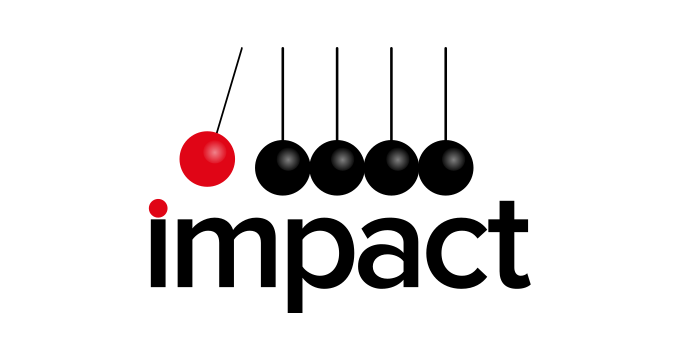
\includegraphics[width=.8\textwidth]{fig/logo}
\end{figure}

This paper discusses the \code{impact} package manager.  The primary
goal of this project is to support the development of a healthy
eco-system around Modelica.  For many other languages, the existence
of an easy to use package manager has made it easier for people to
explore and adopt those languages.  We seek to bring that same kind
of capability to the Modelica community by incorporating useful
features from other package managers like \code{bower}, \code{npm},
\emph{etc.}

This paper is an update on the status of the \code{impact} package
manager which was discussed previously in \parencite{impact1}.  This
latest version of \code{impact} involves a complete rewrite that
incorporates a more advanced dependency resolution algorithm.  That
dependency resolution will be discussed in depth along with many of
the subtle issues that arose during the development of this latest
version of \code{impact}.  Along with a superior dependency resolution
scheme, the new version of \code{impact} is much easier to install
and use.  Furthermore, it includes many useful new features as well.


% References using biblatex
\small
\printbibliography%
\normalsize

\end{document}
